\documentclass{article}
\usepackage{graphicx} 
\usepackage{amsmath}
\usepackage{float}
\graphicspath{{images/}}

\title{\textbf{Power Electronics Laboratory 
\\Session 5: Three-Phase DC-AC Converter}}
\author{Team 3 :
 \\Po Ting Yeh K-9056
\\Beyazit Bilal Ozkaya 341967
 \\Braulio Cardenas 342021}
\date{}

\begin{document}

\maketitle

\section*{Introduction}
This laboratory session investigates the operational principles and modulation strategies of a Three-Phase 2-Level Voltage Source Inverter (VSI). The experiment is divided into two main parts:
\begin{itemize}
    \item Standard Operation: Constructing a Sinusoidal PWM (SPWM) circuit to analyze the relationship between switching states, phase voltages, and active power under various modulation indexes.
\end{itemize}
\begin{itemize}
    \item Advanced Modulation Techniques: Exploring the transition from the linear region to the overmodulation region to observe low-frequency harmonic distortion. Furthermore, the implementation of Third-Harmonic Injection and Min-Max Injection (equivalent to SVPWM) is evaluated. These common-mode injection techniques aim to maximize the DC bus utilization while maintaining a purely sinusoidal load voltage through floating neutral cancellation.
\end{itemize}
\section{Part 1}
\subsection{Task 1:}

\begin{table}[H]
\centering
\begin{tabular}{|c|c|c|c|c|c|c|c|c|}
\hline
State & Sa & Sb & Sc & Van & Vbn & Vab & VaN & VnN \\
\hline
0 & 1 & 0 & 0 & 400  & -200 & 600  & 600 & 200 \\
\hline
1 & 1 & 1 & 1 & 200  & 200  & 0    & 600 & 400 \\
\hline
2 & 0 & 1 & 0 & -200 & 400  & -600 & 0   & 200 \\
\hline
3 & 0 & 1 & 1 & -400 & 200  & -600 & 0   & 400 \\
\hline
4 & 0 & 0 & 1 & -200 & -200 & 0    & 0   & 200 \\
\hline
5 & 1 & 0 & 1 & 200  & -400 & 600  & 600 & 400 \\
\hline
6 & 1 & 1 & 1 & 0    & 0    & 0    & 600 & 600 \\
\hline
7 & 0 & 0 & 0 & 0    & 0    & 0    & 0   & 0 \\
\hline
\end{tabular}
\caption{State Table}
\end{table}

\subsection{Task 2:}
\begin{figure}[H]
    \centering
    
\includegraphics[width=1\linewidth]{img1.png}
    \caption{Topology 3-phase 2-level converter}
    \label{fig:placeholder}
\end{figure}
\subsection{Task 3:}
\subsubsection{Calculation of Modulation Indexes ($m$)}
In a 3-phase SPWM voltage source inverter, the line-to-line RMS voltage ($V_{LL,rms}$) relates to the DC bus voltage ($V_{dc} = 600\text{V}$) and the modulation index ($m$) through the equation:
$$V_{LL,rms} = \sqrt{3} \cdot \frac{m \cdot V_{dc}}{2\sqrt{2}} \approx m \cdot 367.42\text{V}$$
By rearranging the formula, the required modulation indexes are calculated as follows:
\begin{itemize}
    \item For $360\text{V}$: $m = 360 / 367.42 \approx \mathbf{0.980}$
\end{itemize}
\begin{itemize}
    \item For $300\text{V}$: $m = 300 / 367.42 \approx \mathbf{0.816}$
\end{itemize}
\begin{itemize}
    \item For $250\text{V}$: $m = 250 / 367.42 \approx \mathbf{0.680}$
\end{itemize}
\begin{figure}[H]
    \centering
    
\includegraphics[width=0.75\linewidth]{img2.png}
    \caption{m = 0.980}
    \label{fig:placeholder}
\end{figure}
\begin{figure}[H]
    \centering
    
\includegraphics[width=0.75\linewidth]{img3.png}
    \caption{m = 0.816}
    \label{fig:placeholder}
\end{figure}
\begin{figure}[H]
    \centering
    
\includegraphics[width=0.75\linewidth]{img4.png}
    \caption{m = 0.680}
    \label{fig:placeholder}
\end{figure}
\subsubsection{Load Current and Active Power Calculations}
Given the fundamental frequency $f = 50\text{Hz}$, a load inductance of $L = 15\text{mH}$, and a resistance of $R = 15\Omega$, the magnitude of the load impedance is $|Z| = \sqrt{15^2 + (2\pi \cdot 50 \cdot 0.015)^2} = \sqrt{15^2 + 4.71^2} \approx \mathbf{15.72\Omega}$. The RMS phase voltage is calculated as $V_{an,rms} = V_{LL,rms} / \sqrt{3}$.
\\
\\Using these values, the theoretical RMS phase current ($I_{rms} = V_{an,rms} / |Z|$) and the total 3-phase active power ($P = 3 \cdot I_{rms}^2 \cdot R$) are:
\\
\begin{itemize}
    \item Case 1 ($360\text{V}, m_a=0.980$): $V_{an,rms} = 207.85\text{V}$ $\rightarrow$ $I_{rms} = \mathbf{13.22\text{A}}$, $P = \mathbf{7867\text{W}}$
\end{itemize}
\begin{figure}[H]
    \centering
    
\includegraphics[width=1\linewidth]{img5.png}
    \caption{Active Power case 1}
    \label{fig:placeholder}
\end{figure}
\begin{itemize}
    \item Case 2 ($300\text{V}, m_a=0.816$): $V_{an,rms} = 173.21\text{V}$ $\rightarrow$ $I_{rms} = \mathbf{11.02\text{A}}$, $P = \mathbf{5454\text{W}}$
\end{itemize}
\begin{figure}[H]
    \centering
    
\includegraphics[width=1\linewidth]{img6.png}
    \caption{Active Power case 2}
    \label{fig:placeholder}
\end{figure}
\begin{itemize}
    \item Case 3 ($250\text{V}, m_a=0.680$): $V_{an,rms} = 144.34\text{V}$ $\rightarrow$ $I_{rms} = \mathbf{9.18\text{A}}$, $P = \mathbf{3788\text{W}}$
\end{itemize}
\begin{figure}[H]
    \centering
    
\includegraphics[width=1\linewidth]{img7.png}
    \caption{Active Power case 3}
    \label{fig:placeholder}
\end{figure}

\subsubsection{Simulation Verification}
The converter was simulated in PLECS using the calculated $m_a$ values. The measured output voltage relative to the DC negative bus ($v_{aN}$) switches strictly between $0\text{V}$ and $+600\text{V}$. In contrast, the load phase voltage ($v_{an}$) swings symmetrically around $0\text{V}$ with a multi-level stepped waveform. The measured RMS currents and 3-phase active power in the simulation strongly align with the theoretical calculations, successfully validating the SPWM configuration and the power transfer capability.

\subsection{Task 4:}
\begin{figure}[H]
    \centering
    
\includegraphics[width=0.75\linewidth]{img8.png}
    \caption{FFT spectrum of m = 0.98)}
    \label{fig:placeholder}
\end{figure}
As observed in the FFT spectrum, the voltage relative to the DC negative bus ($v_{aN}$) contains a massive DC component (0 Hz) equal to exactly $300\text{V}$, which is $V_{dc}/2$. This occurs because the leg voltage $v_{aN}$ switches strictly between $0\text{V}$ and $+600\text{V}$ with a 50\% duty cycle at the fundamental zero-crossing, resulting in a constant average offset of $300\text{V}$.
\\
\\However, this $300\text{V}$ DC component completely disappears in the load phase voltage ($v_{an}$) and the line-to-line voltage ($v_{ab}$). The justification lies in the balanced three-phase star topology:
\begin{itemize}
    \item Cancellation in Line-to-Line Voltage ($v_{ab}$): All three converter legs ($v_{aN}$, $v_{bN}$, $v_{cN}$) possess the exact same $300\text{V}$ DC offset. Since the line-to-line voltage is the difference between two legs ($v_{ab} = v_{aN} - v_{bN}$), the common DC offsets perfectly cancel each other out ($300\text{V} - 300\text{V} = 0\text{V}$).
\end{itemize}
\begin{itemize}
    \item Cancellation in Phase Voltage ($v_{an}$): In a balanced star-connected load with a floating neutral, the neutral point voltage ($v_{nN}$) represents the instantaneous average of the three leg voltages. Consequently, $v_{nN}$ inherently absorbs this $300\text{V}$ common-mode DC offset. The load phase voltage is defined as $v_{an} = v_{aN} - v_{nN}$. Subtracting the neutral point's $300\text{V}$ bias from the leg's $300\text{V}$ bias entirely eliminates the DC component, leaving a pure AC waveform across the load.
\end{itemize}
\section{Part 2}
\subsection{Task 1:}
\begin{figure}[H]
    \centering
    
\includegraphics[width=0.75\linewidth]{img9.png}
    \caption{m = 0.9}
    \label{fig:placeholder}
\end{figure}
\begin{figure}[H]
    \centering
    
\includegraphics[width=0.75\linewidth]{img10.png}
    \caption{m = 0.95}
    \label{fig:placeholder}
\end{figure}
\begin{figure}[H]
    \centering
    
\includegraphics[width=0.75\linewidth]{img11.png}
    \caption{m = 1.0}
    \label{fig:placeholder}
\end{figure}
\begin{figure}[H]
    \centering
    
\includegraphics[width=0.75\linewidth]{img12.png}
    \caption{m = 1.05}
    \label{fig:placeholder}
\end{figure}
\begin{figure}[H]
    \centering
    
\includegraphics[width=0.75\linewidth]{img13.png}
    \caption{m = 1.1}
    \label{fig:placeholder}
\end{figure}

\subsubsection{Observation of Low-Frequency Component Waveforms:}
By applying a moving average filter tuned to the switching frequency ($f_{sw} = 10\text{kHz}$), the high-frequency switching ripple is removed, revealing the fundamental low-frequency component of the output voltage.
\begin{itemize}
    \item In the \textit{linear region} ($m = 0.90, 0.95, 1.00$), the filtered output voltage remains a pure, undistorted sinusoidal waveform. The amplitude of the fundamental voltage increases linearly with $m$.
\end{itemize}
\begin{itemize}
    \item In the \textbf{over-modulation region} ($m = 1.05, 1.10$), the reference sine wave exceeds the amplitude of the triangular carrier wave. This causes the PWM modulator to stop switching near the peaks of the reference signal, a phenomenon known as "pulse dropping." As a result, the filtered output voltage waveform becomes clipped (flattened at the top and bottom), gradually transitioning from a pure sine wave toward a square wave.
\end{itemize}

\begin{figure}[H]
    \centering
    
\includegraphics[width=0.5\linewidth]{img14.png}
    \caption{Enter Caption}
    \label{fig:placeholder}
\end{figure}
\begin{figure}[H]
    \centering
    
\includegraphics[width=0.5\linewidth]{img15.png}
    \caption{Enter Caption}
    \label{fig:placeholder}
\end{figure}
\begin{figure}[H]
    \centering
    
\includegraphics[width=0.5\linewidth]{img16.png}
    \caption{Enter Caption}
    \label{fig:placeholder}
\end{figure}
\begin{figure}[H]
    \centering
    
\includegraphics[width=0.5\linewidth]{img17.png}
    \caption{Enter Caption}
    \label{fig:placeholder}
\end{figure}
\begin{figure}[H]
    \centering
    
\includegraphics[width=0.5\linewidth]{img18.png}
    \caption{Enter Caption}
    \label{fig:placeholder}
\end{figure}
\subsubsection{Comment on Low-Frequency Harmonics (FFT Analysis 0-1kHz):}
\begin{itemize}
    \item For $m <= 1.0$, the FFT spectrum between 0 and 1 kHz contains almost exclusively the $50\text{Hz}$ fundamental frequency. Low-order harmonics are virtually nonexistent.
\end{itemize}
\begin{itemize}
    \item For $m > 1.0$, the clipping effect introduced by overmodulation severely distorts the waveform, which mathematically generates low-frequency harmonics. Due to the symmetrical nature of the waveform and the absence of a neutral return path in the balanced 3-phase load, triplen harmonics (3rd, 9th, 15th) are inherently suppressed. Consequently, the dominant low-frequency harmonics that emerge in the FFT spectrum are the \textbf{5th(250\text { Hz}), 7th(350 \text{ Hz}), and 11th(550 \text{ Hz}),)}. As $m_a$ increases further into overmodulation, the magnitude of these low-order harmonics grows significantly, which deteriorates the power quality and increases harmonic distortion in the load current.
\end{itemize}
\subsection{Task 2:}
\begin{figure}[H]
    \centering
    
\includegraphics[width=1\linewidth]{img19.png}
    \caption{ Topology of standard PWM with common-mode component}
    \label{fig:placeholder}
\end{figure}
\subsubsection{Theoretical Justification:}

By injecting a third-harmonic component into the fundamental reference signal, the peak of the resultant modulating signal is flattened. The injected modulating signal is defined as:
$$m_{new}(t) = M\sin(\omega t) + \frac{M}{6}\sin(3\omega t)$$
\begin{itemize}
    \item To find the maximum value of this function, we evaluate it at $\omega t = 60^\circ$ (where the peak of the flattened waveform occurs):
\end{itemize}
$$m_{new,max} = M\sin(60^\circ) + \frac{M}{6}\sin(180^\circ) = M\frac{\sqrt{3}}{2}$$
\begin{itemize}
    \item To prevent overmodulation and pulse dropping, the peak of the modulating signal must not exceed the triangular carrier amplitude ($1.0$). Therefore:
\end{itemize}
$$M\frac{\sqrt{3}}{2} \le 1 \implies M \le \frac{2}{\sqrt{3}} \approx 1.154$$
This demonstrates mathematically that the fundamental modulation index ($m_a$) can be increased to approximately $1.15$ without entering the overmodulation region, extending the linear range by $15\%$.
\begin{figure}[H]
    \centering
    
\includegraphics[width=0.5\linewidth]{img20.png}
    \caption{Low-Frequency Output Voltage for Different Modulation Indices}
    \label{fig:placeholder}
\end{figure}
\begin{figure}[H]
    \centering
    
\includegraphics[width=0.5\linewidth]{img21.png}
    \caption{FFT Spectrum of the Output Voltage}
    \label{fig:placeholder}
\end{figure}
\subsubsection{Simulation Verification:}
The third-harmonic injection was implemented in PLECS by adding a $150\text{Hz}$ common-mode sine wave (amplitude $1.15/6$) to the three-phase $50\text{Hz}$ fundamental references (amplitude $1.15$).
\begin{itemize}
    \item \textbf{Modulating Signal:} The resultant reference signal exhibits a saddle shape, effectively keeping its peak within the $[-1, 1]$ bounds.
\end{itemize}
\begin{itemize}
    \item \textbf{Load Phase Voltage and FFT:} Since the injected third-harmonic is a zero-sequence (common-mode) component, it is identical in all three phases and is naturally cancelled out in the line-to-line voltages and absorbed by the floating neutral point. The filtered load phase voltage ($v_{an}$) remains a pure, unclipped sinusoidal waveform. The FFT spectrum verifies that, despite $M = 1.15$, there are no significant low-order harmonics (e.g., 5th or 7th) introduced, successfully avoiding the harmonic distortion typically associated with standard SPWM overmodulation.
\end{itemize}

\subsection{Task 3:}
\begin{figure}[H]
    \centering
    
\includegraphics[width=1\linewidth]{img22.png}
    \caption{Topology of standard PWM with a new common mode component:}
    \label{fig:placeholder}
\end{figure}
\begin{figure}[H]
    \centering
    
\includegraphics[width=0.5\linewidth]{img23.png}
    \caption{Common-Mode V. ($V_n$) under Third-Harmonic and Min-Max Injection Techniques}
    \label{fig:placeholder}
\end{figure}
\subsubsection{Implementation and Waveform Observation:}
The Min-Max injection technique was implemented by calculating the instantaneous common-mode voltage offset using the formula:
$$V_{cm} = -\frac{\max(m_a, m_b, m_c) + \min(m_a, m_b, m_c)}{2}$$
This common-mode signal is then added back to the three fundamental sine waves ($m_{new_x} = m_x + V_{cm}$).
\\
\\Observing the modulating signal $m_{new_a}$ in the simulation reveals a characteristic "double-hump" (camel-back) waveform. This specific injection mathematically centers the active voltage vectors within the carrier bounds at all times, making it identical to the continuous Space Vector PWM (SVPWM) strategy. As observed in the filtered phase voltage ($v_{an}$), the output remains perfectly sinusoidal without any low-frequency harmonic distortion, even when the modulation index is pushed beyond 1.0.
\\
\\ Comparison of DC Bus Utilization:
\begin{itemize}
    \item Standard SPWM: In conventional sinusoidal PWM, the peak of the modulating signal directly corresponds to the fundamental amplitude. The maximum linear modulation index without clipping is $M = 1.0$. The maximum achievable fundamental phase voltage peak is $V_{dc}/2$.
\end{itemize}
\begin{itemize}
    \item Min-Max Injection: By flattening the peaks of the modulating waves, the Min-Max technique allows the fundamental modulation index to be increased up to $M = \frac{2}{\sqrt{3}} \approx 1.1547$ before the flattened peaks hit the triangular carrier limits ($\pm 1.0$).
\end{itemize}
\begin{figure}[H]
    \centering
    
\includegraphics[width=0.75\linewidth]{img24.png}
    \caption{Modulating signal before the Comparator}
    \label{fig:placeholder}
\end{figure}

\\By observing the modulating signal before the comparator, the characteristic double-hump waveform is clearly visible. The Min-Max injection perfectly bounds the peak of the $M=1.15$ reference signal within the $\pm 1.0$ carrier limits, proving how the linear modulation range is extended.
\\
\\\textbf{Comments:}
The Min-Max injection technique seamlessly extends the linear operation region. Compared to standard SPWM, it maximizes the available DC bus utilization by $15.47\%$, allowing the converter to extract more AC voltage from the same DC source while preventing low-order harmonic distortion associated with overmodulation.
\subsection{Task 4:}
\begin{figure}[H]
    \centering
    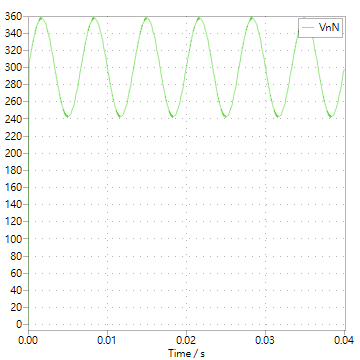
\includegraphics[width=0.5\linewidth]{img25.png}
    \caption{Third-Harmonic injection Common Mode Voltage plot}
    \label{fig:placeholder}
\end{figure}
\begin{figure}[H]
    \centering
    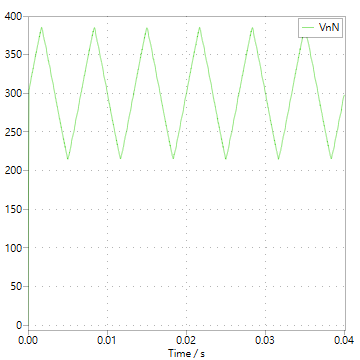
\includegraphics[width=0.5\linewidth]{img26.png}
    \caption{Min-Max injection  Common Mode Voltage plot}
    \label{fig:placeholder}
\end{figure}
\subsubsection{Observation of Common Mode Voltage ($v_{nN}$):}
When measuring the common-mode voltage $v_{nN}$ (the voltage between the load star point and the negative DC bus) with a moving average filter, it becomes evident where the injected distorted signals reside.
\begin{itemize}
    \item In the \textbf{Third-Harmonic injection}, the low-frequency component of $v_{nN}$ contains the standard $300\text{V}$ DC offset ($V_{dc}/2$) superimposed with a distinct $150\text{Hz}$ sinusoidal ripple.
\end{itemize}
\begin{itemize}
    \item In the\textbf{Min-Max injection}, $v_{nN}$ displays the $300\text{V}$ DC offset superimposed with a highly distorted, triangular-like ripple that corresponds directly to the injected $-\frac{\max + \min}{2}$ signal.
\end{itemize}

\subsection{Task 5:}
\subsubsection{Critical Justification (Why load voltage remains perfectly sinusoidal):}
Even though heavily distorted signals are injected into the PWM modulating references to maximize DC bus utilization, the load phase voltage ($v_{an}$) and line currents remain perfectly sinusoidal. This phenomenon is justified by the circuit topology and the nature of the injected signals:
\begin{itemize}
    \item Zero-Sequence Nature: Both the third-harmonic and the Min-Max components are injected identically into all three phases. Therefore, they act strictly as zero-sequence (or common-mode) voltages.
\end{itemize}
\begin{itemize}
    \item Floating Neutral Cancellation: The load is connected in a balanced star (Y) configuration without a physical neutral wire returning to the source (floating neutral). In such a balanced system, the neutral point voltage ($v_{nN}$) is mathematically constrained to be the instantaneous average of the three leg voltages ($v_{aN}, v_{bN}, v_{cN}$). Consequently, the neutral point inherently absorbs the entirety of the injected common-mode signal (along with the $V_{dc}/2$ offset).
\end{itemize}
\begin{itemize}
    \item Differential Output: The actual voltage applied across the load phase is the differential voltage between the converter leg and the neutral point:
\end{itemize}
$$v_{an} = v_{aN} - v_{nN}$$
Because the distorted injected signal exists identically in both $v_{aN}$ and $v_{nN}$, it is perfectly subtracted out in the equation. The common-mode distortion cancels itself completely, leaving only the pure, fundamental $50\text{Hz}$ differential-mode sine wave across the load.

\section*{Conclusion}
This experiment successfully verifies the characteristics and limitations of different modulation techniques in a 3-phase VSI. The key findings are summarized as follows:
\begin{itemize}
    \item \textbf{SPWM and DC Offset:} In standard SPWM, the $V_{dc}/2$ common-mode DC offset generated by the leg voltages is inherently cancelled out in the line-to-line and load phase voltages due to the balanced star-topology.
\end{itemize}
\begin{itemize}
    \item \textbf{Over-modulation Consequences:} Operating the inverter in the over-modulation region ($m_a > 1.0$) causes pulse dropping and waveform clipping, which significantly degrades power quality by introducing low-order harmonics (e.g., 5th and 7th).
\end{itemize}
\begin{itemize}
\item \textbf{DC Bus Utilization Enhancement:} By flattening the modulating signal peaks, both Third-Harmonic and Min-Max Injection successfully extend the linear modulation range to $M \approx 1.1547$. This yields a 15.47\% increase in maximum achievable AC voltage without clipping.
\end{itemize}
\begin{itemize}
    \item \textbf{Floating Neutral Filtering:} Although advanced modulations inject heavily distorted signals (such as saddle or double-hump waveforms), these signals are strictly zero-sequence. They are entirely absorbed by the floating neutral point, ensuring that the differential output across the load remains a pure fundamental sine wave.
\end{itemize}


\end{document}
